% This file is meant to be included in another 
\documentclass{article}
\usepackage{epsfig}
\begin{document}
\section{{\tt Overlap()}}

\subsection{Purpose}
% A short description of purpose. 

Creates a vector structure containing values of the overlap reduction 
function for a pair of interferometers.
The individual interferometer sites currently available are:
%
\begin{itemize}
\item LHO: LIGO Hanford Observatory
\item LLO: LIGO Livingston Observatory
\item VIRGO
\item GEO-600
\item TAMA-300
\end{itemize}
%
One can add additional interferometer sites as needed.

\subsection{Synopsis}
% Syntax: argument definitions, calling signature

\begin{verbatim}
#include "Overlap.h"

void Overlap ( Status *, REAL4Vector *, OverlapParameters * );

typedef struct tagOverlapParameters {
  IFOsite   site1ID;  /* ID number for interferometer site #1 */
  IFOsite   site2ID;  /* ID number for interferometer site #2 */
  INT4      length;   /* length of vector containing overlap red. function */
  REAL4     deltaF;   /* frequency spacing for overlap reduction function */
} OverlapParameters;

typedef enum {
  LHO,      /* LIGO Hanford Observatory    */
  LLO,      /* LIGO Livingston Observatory */
  VIRGO,
  GEO600,
  TAMA300
} IFOsite;
\end{verbatim}

\subsection{Description}
% A longer description of what this routine does

{\tt Overlap()\/} calculates the values of the overlap reduction:
%
\begin{equation}
\gamma(f):={5\over 8\pi}\sum_A\int_{S^2}d\hat\Omega\
e^{i2\pi f\hat\Omega\cdot\Delta \vec x/c}\ 
F_1^A(\hat\Omega)F_2^A(\hat\Omega)\ ,
\label{e:gamma(f)}
\end{equation}
%
where $\hat \Omega$ is a unit vector specifying a direction on the 
two-sphere, $\Delta\vec x:=\vec x_1-\vec x_2$ is the separation vector 
between the central stations of the two interferometer sites, and 
%
\begin{equation}
F_i^A(\hat\Omega):=e_{ab}^A(\hat\Omega)\ d_i^{ab}:=
e_{ab}^A(\hat\Omega)\ {1\over 2}\left(\hat X_i^a\hat X_i^b-
\hat Y_i^a\hat Y_i^b\right)\ 
\label{e:F_i^A}
\end{equation}
%
is the response of the $i$th detector $(i=1,2)$ to the $A=+,\times$ 
polarization.  
Here $\hat X_i^a$ and $\hat Y_i^a$ are unit vectors pointing in the
direction of the two arms of the $i$th detector, and 
$e_{ab}^A(\hat\Omega)$ are the spin-2 polarization tensors for the
$A=+,\times$ polarization states.
The overlap reduction function equals unity for coincident and coaligned 
detectors; it decreases below unity when the detectors are shifted apart 
(so there is a phase shift between the signals in the 
two detectors), or  rotated out of coalignment (so the detectors are 
sensitive to different polarizations).
The overlap reduction function arises naturally when calculating the 
cross-correlated signal due to an isotropic and unpolarized stochastic 
gravity-wave background.

Given a choice of two detector sites, a frequency spacing $\Delta f$,
and the number of desired values $N$, {\tt Overlap()\/} outputs a
vector structure of length $N$ containing the values of $\gamma(f)$ 
evaluated at the discrete frequencies $f_i=i\Delta f$, $i=0,1,\cdots, N-1$.

\subsection{Operating Instructions}
% Detailed usage 

\begin{verbatim}
Status             status; 
REAL4Vector*       vector = NULL;
OverlapParameters  parameters;

/* example choice of input parameters */
parameters.site1ID = LHO;
parameters.site2ID = LLO;
parameters.length  = 10000;
parameters.deltaF  = 1.0;

CreateVector (&status, &vector, parameters.length);

/* calculate values of the overlap reduction function */
Overlap( &status, vector, &parameters );

DestroyVector (&status, &vector);
\end{verbatim}


\subsubsection{Arguments}
% Describe meaning of each argument

\begin{itemize}
\item 
{\tt status\/} is a universal status structure. 
Its contents are initially assigned by {\tt INITSTATUS()\/} and then 
set by {\tt Overlap()\/} on return. 
Non-zero status codes indicate an error condition as specified in 
Table~\ref{t:errors}
\item 
{\tt vector\/} is a pointer of structure type {\tt REAL4Vector}.
The length of the vector must equal {\tt parameters.length\/} or an 
error will occur.
Upon successful return from {\tt Overlap()\/}, vector contains the 
values of the overlap reduction function $\gamma(f)$ evaluated at the
discrete frequencies $f_i:=i\Delta f$, $i=0,1,\cdots, N-1$, where
$\Delta f=${\tt parameters.deltaF\/} and $N=${\tt parameters.length\/}.
\item 
{\tt parameters\/} is a structure of type {\tt OverlapParameters\/}.
The site identification numbers 
{\tt parameters.site1ID\/} and {\tt parameters.site2ID\/} must have 
legitimate enum type {\tt IFOsite} values.
{\tt parameters.length} and {\tt parameter.deltaF} must be positive.
They correspond to the desired length $N$ of the output vector and
the frequency spacing $\Delta f$, in Hz.
\end{itemize}

\subsubsection{Options}

The input parameter structure is required.
The output {\tt vector\/} structure is required. 

\subsubsection{Error conditions}
% What constitutes an error condition? What do the error codes mean?

{\tt Overlap()\/} sets the universal status structure on return. 
Non-zero status codes indicate an error condition. 
Error conditions are described in Table~\ref{t:errors}.

\begin{table}
\hskip -0.7in
\begin{tabular}{|r|l|l|}\hline
status&	status&				Description\\
code&	description&			\\\hline
ENULLP&	{\tt \&parameters==NULL\/}&    Address of parameter structure must be\\
& &                                     non-NULL\\
ENULLV&	{\tt \&vector==NULL}&  		Address of vector pointer must be\\
& &                                     non-NULL\\
ESIZE& 	{\tt parameters.length<=0\/}&  	Length $N$ must be positive\\
EDFREQ&	{\tt parameters.deltaF<=0\/}&   Frequency spacing $\Delta f$ must be positive\\
ESITE&	{\tt parameters.siteID<LHO\/} or {\tt >TAMA300\/}& Site ID must have legitimate enum type\\
ESZMM&	{\tt vector$\rightarrow$length!=parameters.length\/}& Vector lengths must agree\\
ENULLD&	{\tt vector$\rightarrow$data==NULL\/}& Data area of vector must be non-NULL\\
\hline
\end{tabular}
\caption{Error conditions for {\tt Overlap()\/}}
\label{t:errors}
\end{table}
                                
\subsection{Algorithms}
% Describe algorithm by which work is done

As shown in Appendix B of \cite{flanagan} and Sec.~III.B of 
\cite{allenromano}, the overlap reduction function can be written in 
closed form as sum of three spherical Bessel functions:
%
\begin{equation}
\gamma(f)=\rho_1(\alpha)\ d_1^{ab}d_{2ab}
+\rho_2(\alpha)\ d_1^{ab}d_{2a}{}^c s_b s_c
+\rho_3(\alpha)\ d_1^{ab}d_2^{cd}s_a s_b s_c s_d\ ,
\label{e:closed1}
\end{equation}
%
where
%
\begin{equation}
\left[ 
\begin{array}{c}
\rho_1\\
\rho_2\\
\rho_3
\end{array}
\right]
=
{1\over 2\alpha^2}
\left[
\begin{array}{rrr}
 10\alpha^2 & -20\alpha   & 10\\
-20\alpha^2 &  80\alpha   & -100\\
  5\alpha^2 & -50\alpha   & 175
\end{array}
\right]\
\left[
\begin{array}{c}
j_0\\
j_1\\
j_2
\end{array}
\right]\ ,
\label{e:closed2}
\end{equation}
%
$j_0$, $j_1$, and $j_2$ are the standard spherical Bessel functions:
%
\begin{eqnarray}
j_0(\alpha)&=&{\sin\alpha\over\alpha} ,\nonumber\\ 
j_1(\alpha)&=&{\sin\alpha\over\alpha^2}-{\cos\alpha\over\alpha}\ ,
\label{e:closed3}\\ 
j_2(\alpha)&=&3\ {\sin\alpha\over\alpha^3}-3\ {\cos\alpha\over\alpha^2}
-{\sin\alpha\over\alpha}\ ,\nonumber
\end{eqnarray}
%
$\vec s$ is a unit vector pointing in the direction of 
$\Delta \vec x:=\vec x_1-\vec x_2$, and $\alpha:=2\pi f|\Delta\vec x|/c$.

{\tt Overlap()\/} calculates the values of $\gamma(f)$ at the discrete
frequencies $f_i:=i\Delta f$, $i=0,1,\cdots,N-1$ as follows:
%

(i) Gets site location and orientation information for each site.
This information consists of the site ID number, the site name, the 
latitude of the central station measured in degrees North of the 
equator, the longitude of the central station measured in degrees
West of Greenwich, England, the orientation of the first arm of
the detector measured in degrees counter-clockwise from true North,
the orientation of the second arm of the detector, again measured in 
degrees counter-clockwise from true North, and the arm length, in cm.
This information is presently ``hard-wired'' in a static function 
contained in {\tt Overlap.c}.
It may be better in the future to have this information stored in
an external data file, and write a routine that inputs this information 
when needed.

(ii) Using the site location and orientation information, calculates the 
$(x,y,z)$ components (in cm) of the central station, as measured in a
reference frame with the origin at the center of the Earth, the
$z$-axis exiting the North pole, and the $x$-axis passing out of the
line of $0^\circ$ longitude, and the $(x,y,z)$ components of the two
unit vectors pointing in the directions of the two arms of the 
interferometer.
This calculation corrects for oblateness of Earth, using a reference
spheroid with equatorial and polar radii given in Table 4.2 of 
\cite{oblate}.

(iii) Calculates the frequency-independent coefficients 
$d_1^{ab}d_{2ab}$, $d_1^{ab}d_{2a}{}^c s_b s_c$, and 
$d_1^{ab}d_{2a}{}^c s_b s_c$ that appear in Eq.~(\ref{e:closed1}).

(iv) Calculates $\gamma(f)$ at each discrete frequency $f_i:=i\Delta f$,
$i=0,1,\cdots N-1$, using a power series expansion for the spherical 
Bessel functions $j_0(\alpha_i)$, $j_a(\alpha_i)$, $j_2(\alpha_i)$ when
$\alpha_i:=2\pi f_i |\Delta\vec x|/c<0.01$.

\subsection{Accuracy}
% For numerical routines address issues related to accuracy:
% approximations, argument ranges, etc.

The overlap reduction function is calculated in single precision.

\subsection{Tests}
% Describe the tests that are part of the test suite

The program {\tt OverlapTest()\/} tests the function {\tt Overlap()\/}.  
It tests all error conditions listed in Table~\ref{t:errors}.  
It also writes to files the values of the overlap reduction function
for all possible interferometer pairs.
Figures \ref{f:LLOLHO}-\ref{f:TAMA300GEO600} show plots of this data
for the case $N=10000$, $\Delta f= 1.0$ Hz.
%
\begin{figure}[htb!]
\begin{center}
{\epsfig{file=LLOLHO.ps,
angle=-90,width=4in,bbllx=25pt,bblly=50pt,bburx=590pt,bbury=740pt}}
\caption{\label{f:LLOLHO}
Overlap reduction function for the LLO--LHO pair.}
\end{center}
\end{figure}
%
%
\begin{figure}[htb!]
\begin{center}
{\epsfig{file=VIRGOLHO.ps,
angle=-90,width=4in,bbllx=25pt,bblly=50pt,bburx=590pt,bbury=740pt}}
\caption{\label{f:VIRGOLHO}
Overlap reduction function for the VIRGO--LHO pair.}
\end{center}
\end{figure}
%
%
\begin{figure}[htb!]
\begin{center}
{\epsfig{file=VIRGOLLO.ps,
angle=-90,width=4in,bbllx=25pt,bblly=50pt,bburx=590pt,bbury=740pt}}
\caption{\label{f:VIRGOLLO}
Overlap reduction function for the VIRGO--LLO pair.}
\end{center}
\end{figure}
%
%
\begin{figure}[htb!]
\begin{center}
{\epsfig{file=GEO600LHO.ps,
angle=-90,width=4in,bbllx=25pt,bblly=50pt,bburx=590pt,bbury=740pt}}
\caption{\label{f:GEO600LHO}
Overlap reduction function for the GEO600--LHO pair.}
\end{center}
\end{figure}
%
%
\begin{figure}[htb!]
\begin{center}
{\epsfig{file=GEO600LLO.ps,
angle=-90,width=4in,bbllx=25pt,bblly=50pt,bburx=590pt,bbury=740pt}}
\caption{\label{f:GEO600LLO}
Overlap reduction function for the GEO600--LLO pair.}
\end{center}
\end{figure}
%
%
\begin{figure}[htb!]
\begin{center}
{\epsfig{file=GEO600VIRGO.ps,
angle=-90,width=4in,bbllx=25pt,bblly=50pt,bburx=590pt,bbury=740pt}}
\caption{\label{f:GEO600VIRGO}
Overlap reduction function for the GEO600--VIRGO pair.}
\end{center}
\end{figure}
%
%
\begin{figure}[htb!]
\begin{center}
{\epsfig{file=TAMA300LHO.ps,
angle=-90,width=4in,bbllx=25pt,bblly=50pt,bburx=590pt,bbury=740pt}}
\caption{\label{f:TAMA300LHO}
Overlap reduction function for the TAMA300--LHO pair.}
\end{center}
\end{figure}
%
%
\begin{figure}[htb!]
\begin{center}
{\epsfig{file=TAMA300LLO.ps,
angle=-90,width=4in,bbllx=25pt,bblly=50pt,bburx=590pt,bbury=740pt}}
\caption{\label{f:TAMA300LLO}
Overlap reduction function for the TAMA300--LLO pair.}
\end{center}
\end{figure}
%
%
\begin{figure}[htb!]
\begin{center}
{\epsfig{file=TAMA300VIRGO.ps,
angle=-90,width=4in,bbllx=25pt,bblly=50pt,bburx=590pt,bbury=740pt}}
\caption{\label{f:TAMA300VIRGO}
Overlap reduction function for the TAMA300--VIRGO pair.}
\end{center}
\end{figure}
%
%
\begin{figure}[htb!]
\begin{center}
{\epsfig{file=TAMA300GEO600.ps,
angle=-90,width=4in,bbllx=25pt,bblly=50pt,bburx=590pt,bbury=740pt}}
\caption{\label{f:TAMA300GEO600}
Overlap reduction function for the TAMA300--GEO600 pair.}
\end{center}
\end{figure}
%

\subsection{Uses}
% What LLAL, other routines does this one call?

{\tt InitStatus()\/}, 
{\tt dCreateVector()\/} if {\tt vector==NULL}, and
{\tt StatusHandler()\/}.

\subsection{Notes}
% Miscellaneous notes that do not appear elsewhere. Things remaining
% to be done, etc. 

\begin{itemize}
%
\item
The header file {\tt Overlap.h\/} defines a macro
%
\begin{verbatim}
#define NUMBEROFSITES (int(TAMA300+1))
\end{verbatim}
%
This macro can be used, e.g, to loop over different pairs of 
interferometer sites.
Since the number of interferometer sites is expected to change in the 
future, {\tt NUMBEROFSITES\/} should always be used in place of an 
explicit integer.
\item
There is an error in Eq.~(B6) of Ref.~\cite{flanagan}; 
the factor multiplying $j_1(\alpha)$ in the expression for 
$\rho_1(\alpha)$ should be $-10/\alpha$, not $-2/\alpha$.
This error was corrected in the Eq.~(\ref{e:closed2}) above.
\item
It may be useful, in the future, to extend ${\tt Overlap()\/}$ to 
calculate the overlap reduction for a pair of acoustic resonant
detectors and/or for interferometer--acoustic resonant detector pairs.
%
\end{itemize}

\subsection{References}
% Any references for algorithms, tests, etc.

\begin{thebibliography}{0}
\bibitem{flanagan}
E.~Flanagan, 
Phys.\ Rev.\ D.\ {\bf 48}, 2389 (1993).
\bibitem{allenromano}
B.~Allen and J.D.~Romano, 
Phys.\ Rev.\ D.\ {\bf 59}, 102001 (1999).
\bibitem{oblate}
"Spacecraft attitude determination and control,''  
Ed.\ James R.\ Wertz, 
(D.\ Reidel Publishing Co., Boston, 1978).
\end{thebibliography}


\end{document}
